\newpage
\section{Teoria de funcionamento}

\subsection{Circuito de proteção contra sobre tensão}

\subsubsection{Utilizando diodo Zener}

Analisando o circuito da figura \ref{f_zener}, quando a tensão $V_{in}$ se torna maior que $V_z$, o diodo $D_z$ passa a conduzir, fazendo com que haja uma queda de tensão em $R_z$ igual a $V_{rz} = V_{in} - V_z$. Isso faz com que a tensão em $V_o$ seja mantida constante em, no máximo $V_z$. A equação \ref{e_rz} é, então, utilizada para calcular o valor de $R_z$ de modo a evitar a queima do diodo, onde $I_{zmax}$ é a corrente máxima permitida no diodo.

\begin{equation}
V_{rz} \ge \frac{V_{in} - V_z}{I_{zmax}}
\label{e_rz}
\end{equation}

\begin{figure}[H]
    \centering
    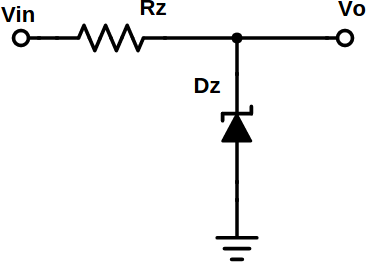
\includegraphics[scale=0.4]{img/zener.png}
    \caption{Circuito para proteção de sobre tensão utilizando diodo zener.}
    \label{f_zener}
\end{figure}

\subsubsection{Utilizando diodo Convercional}
 O circuito da figura \ref{f_diodo} possui um princípio de operação semelhante, quando $V_{in}$ é mair que $V_d + V_{cc}$ ou menor que $-V_d$, os diodos conduzem. Porém, diferente do circuito com zener, este necessita de 2 diodos para proteção contra tensões abaixo de 0 V.
 
 A equação \ref{e_R1} é utilizada para o calculo do resistor $R_1$. Vale notar que os diodos $D_1$ e $D_2$ devem ser iguais.
 
 \begin{equation}
 R \ge \frac{V_{in} - V_{cc} - V_d}{I_{dmax}}
 \label{e_R1}
 \end{equation}
 
\begin{figure}[H]
	\centering
	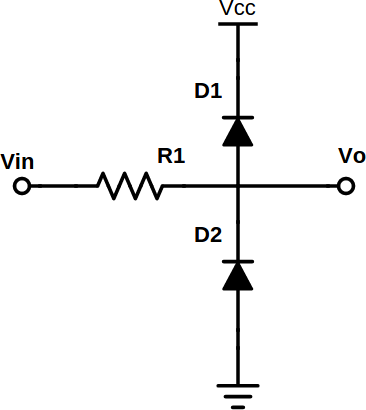
\includegraphics[scale=0.4]{img/diodo.png}
	\caption{Circuito para proteção de sobre tensão utilizando diodo convencional.}
	\label{f_diodo}
\end{figure}

\subsection{Condicionamento de sensor termo-resistivo com corrente constante}
O circuito da figura \ref{f_thermistor} é utilizado para manter uma corrente constante no termistor $R_T$. Note que a tensão no emissor de $Q_1$ é ajustada pelo potenciômetro $P_1$, sendo denominada $V_{ref}$. Assim, a corrente que passa e $R_T$ é

\begin{equation}
I_s = \frac{V_{cc}-V_{ref}}{R_1}.
\label{e_is}
\end{equation}

\begin{figure}[H]
	\centering
	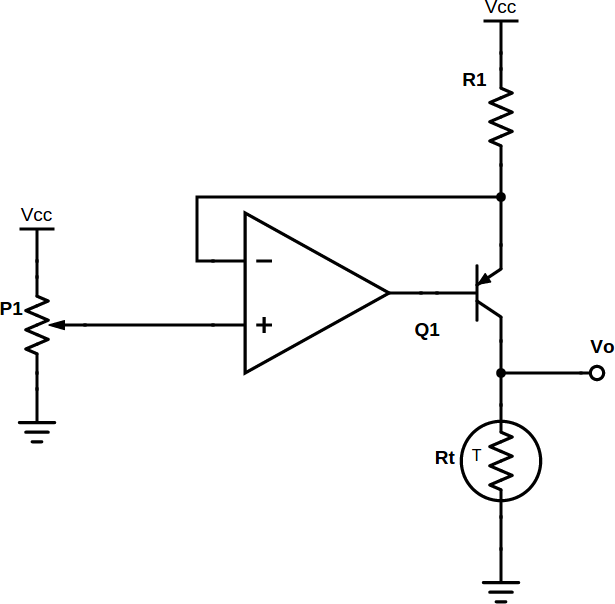
\includegraphics[scale=0.3]{img/thermistor.png}
	\caption{Circuito para condicionamento de sensor de temperatura do tipo termistor.}
	\label{f_thermistor}
\end{figure}